\chapter{Environment Representation}
\label{chp:ER}
\acresetall
This Chapter describes the thought process behind the environment representation. Section \ref{sec:ER-bg} gives relevant background information and context for the problem, and Section \ref{sec:ER-ED} describes how this information is used to formulate a discrete environment representation. Lastly, Section \ref{sec:ER-App} shows a few practical scenarios using this strategy with different on-board cameras. 

\section{Background}
\label{sec:ER-bg}
\subsection{Assumptions}
The goal of this paper is to develop a coverage path planning algorithm \hbox{applicable} in a \ac{sar} situation, using \acp{uav}. To achieve success in such an application, the first step would be to find a way to represent the environment. Essentially, the context in which the \acp{uav} exist needs to be described in some way for them to navigate it successfully.
 
% Offline
The starting assumption is that an offline approach is sufficient. This implies that there is always enough information known about the environment to represent it fully prior to the execution of the path planning algorithm. At the altitude that a \ac{uav} flies, it is reasonable to assume that any obstructions, for example power lines or mountains, can be mapped out a priori. Moreover, \ac{sar} operations often have fixed geographical bounds in which to search.

% No dynamic obstacles or moving target
% TODO: Justify why the target is not assumed to be in motion
Furthermore, it is also assumed that there are no transients in the environment, such as a moving target or dynamic obstacles. Search and rescue operations will rarely have moving elements at the altitude of the \acp{uav}. They are more likely to have fixed no fly zones and static obstacles.

% Two dimensional
Because they are airborne vehicles,\acp{uav} can execute three dimensional movements, which implies the necessity for a three dimensional representation of the environment. In this paper however, it is assumed that altitude changes are not necessary to search an area. Assuming that there is some form of camera on-board the \ac{uav}, a constant altitude will be an advantage. It means that the \ac{gsd} will remain roughly constant, which is a widely accepted measure of camera accuracy. Assuming a camera is on a \ac{uav} pointing down towards the ground, \ac{gsd} is the distance on the ground as represented by the width of one pixel in an image \cite{PropellerAero2021}.

Without altitude changes, \ac{uav} motions can be represented in two-dimensional space, which greatly simplifies the problem. For offline coverage path planning, it is important to have some demarcated two-dimensional region that requires coverage. The identified region, or environment, can be represented in either a discrete or continuous manner. 

% Discrete
% TODO: Mention drawbacks of continuous implementations
% TODO: Mention reasons for choosing discrete - wavefront planner paper pg 674 "An exact cell decomposition is ineffiecient because we are interested in acquiring an equally sized set of images"
In the context of \ac{sar}, complete coverage is very important. It will ensure that every possible point in the environment map is covered. In this scenario, it implies that the camera will have viewed all points on the map. Achieving completeness is by no means trivial, but is more achievable in complex environments when using a discrete approach.

\subsection{Discretisation Using Cameras}
Discretising the environment can be done in a few different ways. Assuming a generic \ac{uav} with some thermal or visual camera on-board, one has a few options. One can discretise the area based on the \ac{uav} size, but a more common practice is to base it off the tool size. In this case, that would be the \ac{fov} of the on-board camera. This also makes the process of complete coverage easier, because if the camera is guaranteed to see the entirety of each discrete cell, it is a complete algorithm so long as each cell is visited.

Therefore, to discretise the environment, the \ac{fov} needs to be calculated. The camera specifications and \ac{uav} altitude will be the determining factors to calculate the \ac{fov}. The type of camera and the flight altitude are design decisions and will depend on the \ac{gsd} necessary to realistically be able to locate the target in a \ac{sar} operation.

The diagram in Figure \ref{fig:FOV} shows all the relevant variables needed to calculate the \acl{fov} along one dimension ($FOV_x$). A similar diagram can be used to calculate the \acl{fov} along the other dimension ($FOV_y$). The only difference would be the sensor size variable, which changes from the sensor width ($w_{len}$) to the sensor height ($h_{len}$). The other variables include the focal length of the camera ($f$), the height of the lens above ground ($H$) and the camera's angle of view ($AOV$). Lastly, there is the variable $\phi$ which is an angle created due to the sensor being slightly smaller than the diameter of the cone of light projected onto it.

The resulting \acl{fov} will be a rectangle of the same aspect ratio of the camera sensor, provided the camera is pointing directly down and the ground is level. For this application, it is assumed the camera is always pointing downwards. This can be accomplished when the \acs{uav} banks by placing the camera on a gimble. The assumption that the ground is level is not entirely reasonable, for example, in a mountainous region. This can be addressed by adding overlap between images to add some redundant coverage, which will be added in Chapter \ref{chp:refuelling}. Doing a topographical inspection is beyond the scope of this project and will not be addressed in more detail.
% TODO: Check this reference and decide whether to include last sentence
\tikzset{every picture/.style={line width=0.75pt}} %set default line width to 0.75pt          
\begin{figure}[h!]
	\centering	      
	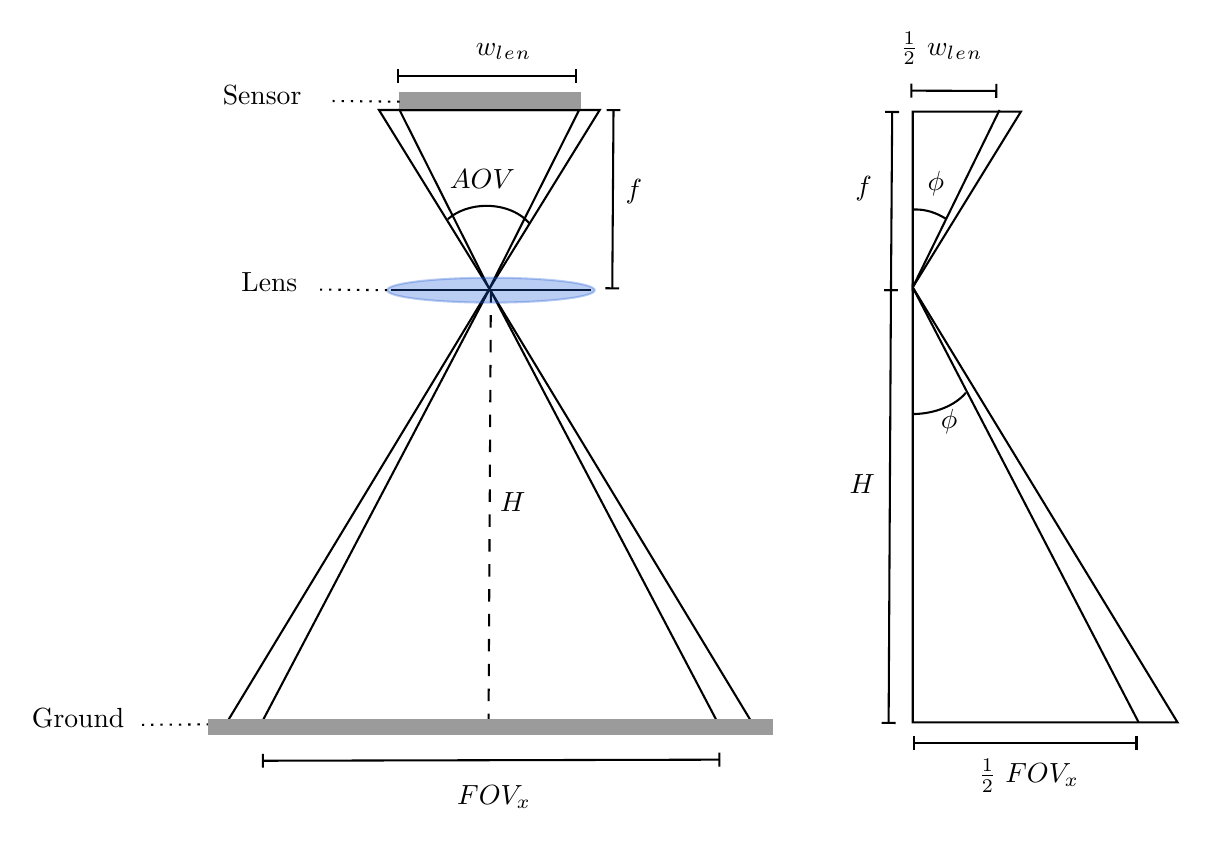
\begin{tikzpicture}[x=0.75pt,y=0.75pt,yscale=-1,xscale=1]
		%uncomment if require: \path (0,445); %set diagram left start at 0, and has height of 445
		
		%Shape: Triangle [id:dp7279031821934365] 
		\draw   (292.52,162.29) -- (239.35,76.17) -- (345.69,76.17) -- cycle ;
		%Shape: Triangle [id:dp08500924272014787] 
		\draw   (292.52,162.29) -- (419.57,372.17) -- (165.48,372.17) -- cycle ;
		%Straight Lines [id:da9387157545116658] 
		\draw    (245.26,162.97) -- (341.26,162.97) ;
		%Shape: Triangle [id:dp15441481766796317] 
		\draw   (292.52,162.29) -- (249.26,76.17) -- (335.78,76.17) -- cycle ;
		%Shape: Triangle [id:dp8187279481172025] 
		\draw   (292.69,162.29) -- (403,372.17) -- (182.39,372.17) -- cycle ;
		%Straight Lines [id:da06491692932377724] 
		\draw    (248.39,59.69) -- (334.14,59.69) ;
		\draw [shift={(334.14,59.69)}, rotate = 180] [color={rgb, 255:red, 0; green, 0; blue, 0 }  ][line width=0.75]    (0,3.35) -- (0,-3.35)   ;
		\draw [shift={(248.39,59.69)}, rotate = 180] [color={rgb, 255:red, 0; green, 0; blue, 0 }  ][line width=0.75]    (0,3.35) -- (0,-3.35)   ;
		%Straight Lines [id:da8254572040663344] 
		\draw    (352.34,76.22) -- (351.75,162.07) ;
		\draw [shift={(351.75,162.07)}, rotate = 270.39] [color={rgb, 255:red, 0; green, 0; blue, 0 }  ][line width=0.75]    (0,3.35) -- (0,-3.35)   ;
		\draw [shift={(352.34,76.22)}, rotate = 270.39] [color={rgb, 255:red, 0; green, 0; blue, 0 }  ][line width=0.75]    (0,3.35) -- (0,-3.35)   ;
		%Straight Lines [id:da18153445552160163] 
		\draw  [dash pattern={on 4.5pt off 4.5pt}]  (293.26,162.97) -- (292.13,371.48) ;
		%Shape: Right Triangle [id:dp9464990257102419] 
		\draw   (548.64,76.92) -- (496.5,161.6) -- (496.5,76.94) -- cycle ;
		%Straight Lines [id:da9593228177444686] 
		\draw    (496.5,161.6) -- (538.33,76.17) ;
		%Shape: Arc [id:dp3427993390498929] 
		\draw  [draw opacity=0] (496.65,124.11) .. controls (496.93,124.1) and (497.22,124.09) .. (497.5,124.09) .. controls (502.76,124) and (507.83,125.61) .. (512.56,128.62) -- (498.77,204.83) -- cycle ; \draw   (496.65,124.11) .. controls (496.93,124.1) and (497.22,124.09) .. (497.5,124.09) .. controls (502.76,124) and (507.83,125.61) .. (512.56,128.62) ;
		%Straight Lines [id:da5534147172451449] 
		\draw    (495.86,66.85) -- (536.76,66.97) ;
		\draw [shift={(536.76,66.97)}, rotate = 180.17] [color={rgb, 255:red, 0; green, 0; blue, 0 }  ][line width=0.75]    (0,3.35) -- (0,-3.35)   ;
		\draw [shift={(495.86,66.85)}, rotate = 180.17] [color={rgb, 255:red, 0; green, 0; blue, 0 }  ][line width=0.75]    (0,3.35) -- (0,-3.35)   ;
		%Straight Lines [id:da49349314045709525] 
		\draw    (486.61,77.11) -- (486.02,162.96) ;
		\draw [shift={(486.02,162.96)}, rotate = 270.39] [color={rgb, 255:red, 0; green, 0; blue, 0 }  ][line width=0.75]    (0,3.35) -- (0,-3.35)   ;
		\draw [shift={(486.61,77.11)}, rotate = 270.39] [color={rgb, 255:red, 0; green, 0; blue, 0 }  ][line width=0.75]    (0,3.35) -- (0,-3.35)   ;
		%Shape: Arc [id:dp09088039941092019] 
		\draw  [draw opacity=0] (272.52,128.74) .. controls (277.02,124.82) and (283.7,122.33) .. (291.17,122.33) .. controls (300.03,122.33) and (307.8,125.84) .. (312.1,131.09) -- (291.17,140.58) -- cycle ; \draw   (272.52,128.74) .. controls (277.02,124.82) and (283.7,122.33) .. (291.17,122.33) .. controls (300.03,122.33) and (307.8,125.84) .. (312.1,131.09) ;
		%Shape: Right Triangle [id:dp9191394953697831] 
		\draw   (496.5,161.6) -- (624.06,371.17) -- (496.5,371.17) -- cycle ;
		%Straight Lines [id:da9606752421348479] 
		\draw    (605.33,371.17) -- (496.5,161.6) ;
		%Shape: Arc [id:dp6813474716985082] 
		\draw  [draw opacity=0] (522.1,212.41) .. controls (516.97,218.5) and (507.3,222.62) .. (496.19,222.67) -- (496,202.42) -- cycle ; \draw   (522.1,212.41) .. controls (516.97,218.5) and (507.3,222.62) .. (496.19,222.67) ;
		%Straight Lines [id:da806740169220673] 
		\draw    (183.39,389.69) -- (403.33,389.17) ;
		\draw [shift={(403.33,389.17)}, rotate = 539.86] [color={rgb, 255:red, 0; green, 0; blue, 0 }  ][line width=0.75]    (0,3.35) -- (0,-3.35)   ;
		\draw [shift={(183.39,389.69)}, rotate = 539.86] [color={rgb, 255:red, 0; green, 0; blue, 0 }  ][line width=0.75]    (0,3.35) -- (0,-3.35)   ;
		%Straight Lines [id:da8133225602503578] 
		\draw    (497.33,381.17) -- (604.33,381.17) ;
		\draw [shift={(604.33,381.17)}, rotate = 180] [color={rgb, 255:red, 0; green, 0; blue, 0 }  ][line width=0.75]    (0,3.35) -- (0,-3.35)   ;
		\draw [shift={(497.33,381.17)}, rotate = 180] [color={rgb, 255:red, 0; green, 0; blue, 0 }  ][line width=0.75]    (0,3.35) -- (0,-3.35)   ;
		%Straight Lines [id:da25053349814928394] 
		\draw    (486.02,162.96) -- (484.89,371.47) ;
		\draw [shift={(484.89,371.47)}, rotate = 270.31] [color={rgb, 255:red, 0; green, 0; blue, 0 }  ][line width=0.75]    (0,3.35) -- (0,-3.35)   ;
		\draw [shift={(486.02,162.96)}, rotate = 270.31] [color={rgb, 255:red, 0; green, 0; blue, 0 }  ][line width=0.75]    (0,3.35) -- (0,-3.35)   ;
		%Shape: Rectangle [id:dp5196090784877698] 
		\draw  [color={rgb, 255:red, 155; green, 155; blue, 155 }  ,draw opacity=1 ][fill={rgb, 255:red, 155; green, 155; blue, 155 }  ,fill opacity=1 ] (249.26,68.14) -- (336,68.14) -- (336,75.17) -- (249.26,75.17) -- cycle ;
		%Shape: Ellipse [id:dp39537204861922115] 
		\draw  [color={rgb, 255:red, 26; green, 88; blue, 211 }  ,draw opacity=0.3 ][fill={rgb, 255:red, 26; green, 88; blue, 211 }  ,fill opacity=0.3 ] (243.26,162.97) .. controls (243.26,159.66) and (265.64,156.97) .. (293.26,156.97) .. controls (320.87,156.97) and (343.26,159.66) .. (343.26,162.97) .. controls (343.26,166.29) and (320.87,168.97) .. (293.26,168.97) .. controls (265.64,168.97) and (243.26,166.29) .. (243.26,162.97) -- cycle ;
		%Shape: Boxed Line [id:dp7067135001640237] 
		\draw  [dash pattern={on 0.84pt off 2.51pt}]  (243.26,162.97) -- (211,162.67) ;
		%Straight Lines [id:da962687715126145] 
		\draw  [dash pattern={on 0.84pt off 2.51pt}]  (157.48,372.17) -- (125.22,372.37) ;
		%Shape: Boxed Line [id:dp25644897900816477] 
		\draw  [dash pattern={on 0.84pt off 2.51pt}]  (249.26,72.14) -- (217,71.84) ;
		%Straight Lines [id:da9121328450253205] 
		\draw [color={rgb, 255:red, 155; green, 155; blue, 155 }  ,draw opacity=1 ][line width=6]    (157.17,373.35) -- (429.09,373.35) ;
		
		% Text Node
		\draw (277.85,37.29) node [anchor=north west][inner sep=0.75pt]  [font=\normalsize]  {$ \begin{array}{l}
				w_{l}{}_{e}{}_{n}\\
			\end{array}$};
		% Text Node
		\draw (171.59,152.9) node [anchor=north west][inner sep=0.75pt]  [font=\normalsize] [align=left] {Lens};
		% Text Node
		\draw (356.67,108.27) node [anchor=north west][inner sep=0.75pt]  [font=\normalsize]  {$f$};
		% Text Node
		\draw (296.25,259.08) node [anchor=north west][inner sep=0.75pt]  [font=\normalsize]  {$H$};
		% Text Node
		\draw (272.06,103.36) node [anchor=north west][inner sep=0.75pt]  [font=\normalsize]  {$AOV$};
		% Text Node
		\draw (502.19,104.3) node [anchor=north west][inner sep=0.75pt]  [font=\normalsize]  {$\phi $};
		% Text Node
		\draw (467.33,106.6) node [anchor=north west][inner sep=0.75pt]  [font=\normalsize]  {$f$};
		% Text Node
		\draw (489,37) node [anchor=north west][inner sep=0.75pt]    {$\frac{1}{2} \ w_{l}{}_{e}{}_{n}$};
		% Text Node
		\draw (508.52,218.96) node [anchor=north west][inner sep=0.75pt]  [font=\normalsize]  {$\phi $};
		% Text Node
		\draw (268.85,398.07) node [anchor=north west][inner sep=0.75pt]  [font=\normalsize]  {$ \begin{array}{l}
				FOV_{x}\\
			\end{array}$};
		% Text Node
		\draw (520,387.4) node [anchor=north west][inner sep=0.75pt]  [font=\normalsize]  {$ \begin{array}{l}
				\frac{1}{2} \ FOV_{x}\\
			\end{array}$};
		% Text Node
		\draw (464.59,250.41) node [anchor=north west][inner sep=0.75pt]  [font=\normalsize]  {$H$};
		% Text Node
		\draw (162.59,62.9) node [anchor=north west][inner sep=0.75pt]  [font=\normalsize] [align=left] {Sensor};
		% Text Node
		\draw (70.59,363) node [anchor=north west][inner sep=0.75pt]  [font=\normalsize] [align=left] {Ground};
		
		
	\end{tikzpicture}
	\caption{Diagram showing relevant variables concerned with calculating the Field of View for a camera.}
	\label{fig:FOV}
\end{figure}
The calculations required to do a discretisation based on the camera \ac{fov} will now be discussed. The first equation that is required is the calculation of the angle $\phi$ which makes use of the small triangle:
\begin{equation}
	\label{eqn:phi}
	\begin{aligned}
		\tan{\phi} &= \frac{\frac{1}{2}w_{len}}{f} &\\
		\phi &= \tan^{-1}{(\frac{w_{len}}{2f})}
	\end{aligned}	
\end{equation}
Now that $\phi$ is known, the bigger triangle is used to calculate $FOV_x$:
\begin{equation}
	\label{eqn:fov_x}
	\begin{aligned}
		\frac{FOV_x}{2} &= H \times \tan{\phi} &\\
		FOV_x &= 2H \times \tan{ (\tan^{-1}{ (\frac{w_{len}}{2f}) }) } &\\
		FOV_x &= H \times \frac{w_{len}}{f} &\\
	\end{aligned}
\end{equation}
Similarly, $FOV_y$ can be calculated using the other sensor size dimension $h_{len}$:
\begin{equation}
	\label{eqn:fov_y}
	\begin{aligned}
		FOV_y &= H \times \frac{h_{len}}{f}
	\end{aligned}
\end{equation}
Both $FOV_x$ and $FOV_y$ will have the same units as $H$, which is metres. The resolution of the camera is the number of pixels along the image width ($px_w$) multiplied with the number of pixels along its height ($px_h$). These can be used to calculate the $GSD$ by dividing either $FOV$ by the pixel value associated with that dimension:
\begin{equation}
	\label{eqn:GSD}
	\begin{aligned}
		GSD &= \frac{100FOV_x}{px_w} &\\
		GSD &= \frac{100H \times w_{len}}{f \times px_w}
	\end{aligned}
\end{equation}

\section{Discretisation Methodology}
\label{sec:ER-ED}
If the size of the environment discretisation is set equal to the rectangular camera field of view, and the type of camera used is known, then a desired $GSD$ can be used to decide on an appropriate flying height. Choosing a $GSD$ would depend on the application, seen as it represents the level of detail that can potentially be detected in an image.\\
Taking the conservative approach, the assumption is that one is looking for a human being standing upright, viewed from above. To get a good estimate of the space occupied by a human in this orientation, one needs anthropometric data. A survey was done in Europe for people between the ages of 18 and 60 \cite{Jurgens1998}. Among other measurements, they measured chest depth ($w$) and elbow-to-elbow length ($l$). These dimensions represent those of an upright human from above and can be seen in Figure \ref{fig:GSD}.\\ 
\tikzset{every picture/.style={line width=0.75pt}} %set default line width to 0.75pt        
\begin{figure}
	\centering
	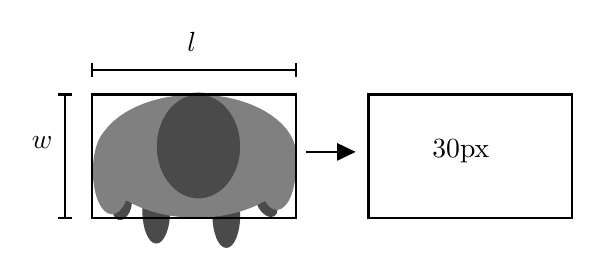
\begin{tikzpicture}[x=0.75pt,y=0.75pt,yscale=-1,xscale=1]
		%uncomment if require: \path (0,300); %set diagram left start at 0, and has height of 300
		
		%Shape: Ellipse [id:dp5061908839346234] 
		\draw  [color={rgb, 255:red, 74; green, 74; blue, 74 }  ,draw opacity=1 ][fill={rgb, 255:red, 74; green, 74; blue, 74 }  ,fill opacity=1 ] (394.62,193.23) .. controls (392.81,189.9) and (392.91,186.34) .. (394.85,185.28) .. controls (396.79,184.23) and (399.83,186.07) .. (401.65,189.41) .. controls (403.47,192.74) and (403.37,196.3) .. (401.43,197.36) .. controls (399.49,198.41) and (396.44,196.57) .. (394.62,193.23) -- cycle ;
		%Shape: Ellipse [id:dp4772697686098053] 
		\draw  [color={rgb, 255:red, 74; green, 74; blue, 74 }  ,draw opacity=1 ][fill={rgb, 255:red, 74; green, 74; blue, 74 }  ,fill opacity=1 ] (324.6,191.47) .. controls (325.46,187.77) and (327.9,185.18) .. (330.05,185.68) .. controls (332.2,186.18) and (333.25,189.58) .. (332.4,193.28) .. controls (331.54,196.98) and (329.1,199.57) .. (326.95,199.07) .. controls (324.8,198.57) and (323.75,195.17) .. (324.6,191.47) -- cycle ;
		%Shape: Ellipse [id:dp7464833674207887] 
		\draw  [color={rgb, 255:red, 74; green, 74; blue, 74 }  ,draw opacity=1 ][fill={rgb, 255:red, 74; green, 74; blue, 74 }  ,fill opacity=1 ] (372.5,196.92) .. controls (372.5,188.32) and (375.28,181.35) .. (378.71,181.35) .. controls (382.13,181.35) and (384.91,188.32) .. (384.91,196.92) .. controls (384.91,205.53) and (382.13,212.5) .. (378.71,212.5) .. controls (375.28,212.5) and (372.5,205.53) .. (372.5,196.92) -- cycle ;
		%Shape: Ellipse [id:dp9681716059666354] 
		\draw  [color={rgb, 255:red, 74; green, 74; blue, 74 }  ,draw opacity=1 ][fill={rgb, 255:red, 74; green, 74; blue, 74 }  ,fill opacity=1 ] (338.74,194.85) .. controls (338.74,186.24) and (341.52,179.27) .. (344.95,179.27) .. controls (348.37,179.27) and (351.15,186.24) .. (351.15,194.85) .. controls (351.15,203.45) and (348.37,210.42) .. (344.95,210.42) .. controls (341.52,210.42) and (338.74,203.45) .. (338.74,194.85) -- cycle ;
		%Shape: Ellipse [id:dp7224271801321214] 
		\draw  [color={rgb, 255:red, 128; green, 128; blue, 128 }  ,draw opacity=1 ][fill={rgb, 255:red, 128; green, 128; blue, 128 }  ,fill opacity=1 ] (316.38,168.78) .. controls (316.38,152.66) and (337.79,139.6) .. (364.19,139.6) .. controls (390.59,139.6) and (412,152.66) .. (412,168.78) .. controls (412,184.9) and (390.59,197.96) .. (364.19,197.96) .. controls (337.79,197.96) and (316.38,184.9) .. (316.38,168.78) -- cycle ;
		%Shape: Ellipse [id:dp3950279689736771] 
		\draw  [color={rgb, 255:red, 128; green, 128; blue, 128 }  ,draw opacity=1 ][fill={rgb, 255:red, 74; green, 74; blue, 74 }  ,fill opacity=1 ] (365.29,138.6) .. controls (376.67,138.6) and (385.9,150.04) .. (385.9,164.15) .. controls (385.9,178.25) and (376.67,189.69) .. (365.29,189.69) .. controls (353.9,189.69) and (344.67,178.25) .. (344.67,164.15) .. controls (344.67,150.04) and (353.9,138.6) .. (365.29,138.6) -- cycle ;
		%Shape: Ellipse [id:dp14441581895383182] 
		\draw  [color={rgb, 255:red, 128; green, 128; blue, 128 }  ,draw opacity=1 ][fill={rgb, 255:red, 128; green, 128; blue, 128 }  ,fill opacity=1 ] (314.91,176.05) .. controls (314.91,164.87) and (318.8,155.8) .. (323.6,155.8) .. controls (328.4,155.8) and (332.29,164.87) .. (332.29,176.05) .. controls (332.29,187.23) and (328.4,196.3) .. (323.6,196.3) .. controls (318.8,196.3) and (314.91,187.23) .. (314.91,176.05) -- cycle ;
		%Shape: Ellipse [id:dp8509174208950578] 
		\draw  [color={rgb, 255:red, 128; green, 128; blue, 128 }  ,draw opacity=1 ][fill={rgb, 255:red, 128; green, 128; blue, 128 }  ,fill opacity=1 ] (394.35,173.97) .. controls (394.35,162.79) and (398.24,153.72) .. (403.03,153.72) .. controls (407.83,153.72) and (411.72,162.79) .. (411.72,173.97) .. controls (411.72,185.16) and (407.83,194.22) .. (403.03,194.22) .. controls (398.24,194.22) and (394.35,185.16) .. (394.35,173.97) -- cycle ;
		%Shape: Rectangle [id:dp6763821992887933] 
		\draw  [line width=0.75]  (314.19,139.1) -- (412.19,139.1) -- (412.19,198.46) -- (314.19,198.46) -- cycle ;
		%Straight Lines [id:da0050447787628182805] 
		\draw    (314.19,127.1) -- (412.19,127.1) ;
		\draw [shift={(412.19,127.1)}, rotate = 180] [color={rgb, 255:red, 0; green, 0; blue, 0 }  ][line width=0.75]    (0,3.35) -- (0,-3.35)   ;
		\draw [shift={(314.19,127.1)}, rotate = 180] [color={rgb, 255:red, 0; green, 0; blue, 0 }  ][line width=0.75]    (0,3.35) -- (0,-3.35)   ;
		%Shape: Rectangle [id:dp8520376009638861] 
		\draw  [line width=0.75]  (447.19,139.1) -- (545.19,139.1) -- (545.19,198.46) -- (447.19,198.46) -- cycle ;
		%Straight Lines [id:da004734927691815605] 
		\draw    (417,166.75) -- (438,166.75) ;
		\draw [shift={(441,166.75)}, rotate = 540] [fill={rgb, 255:red, 0; green, 0; blue, 0 }  ][line width=0.08]  [draw opacity=0] (8.93,-4.29) -- (0,0) -- (8.93,4.29) -- cycle    ;
		%Straight Lines [id:da5120965397340576] 
		\draw    (301.19,139.1) -- (301.19,198.46) ;
		\draw [shift={(301.19,198.46)}, rotate = 270] [color={rgb, 255:red, 0; green, 0; blue, 0 }  ][line width=0.75]    (0,3.35) -- (0,-3.35)   ;
		\draw [shift={(301.19,139.1)}, rotate = 270] [color={rgb, 255:red, 0; green, 0; blue, 0 }  ][line width=0.75]    (0,3.35) -- (0,-3.35)   ;
		
		% Text Node
		\draw (358.5,107.4) node [anchor=north west][inner sep=0.75pt]    {$l$};
		% Text Node
		\draw (283.5,157.9) node [anchor=north west][inner sep=0.75pt]    {$w$};
		% Text Node
		\draw (476.5,159.5) node [anchor=north west][inner sep=0.75pt]   [align=left] {30px};		
	\end{tikzpicture}
	\caption{Figure showing the rectangular approximation for a human viewed from above for calculation of the GSD}
	\label{fig:GSD}
\end{figure}
To calculate \acs{gsd}, a minimum number of pixels needed to make a human visible must be chosen. There is an article wherein they developed an image processing algorithm for human detection in a \acl{sar} scenario \cite{Rudol2008}. In this article they made the decision to put a 30 pixel requirement on human detection.
% TODO: Maybe refer back to the literature review where the Rudol paper should be mentioned for the first time.
Figure \ref{fig:GSD} shows the rectangular approximation for a human that the 30 pixels should represent.\\
Using the lower percentile measurements of 170mm chest depth and 390mm elbow-to-elbow length along with the 30 pixel requirement, one gets a \ac{gsd} of roughly 4.7cm/px. For a child, these values could be even smaller. Therefore, 4cm/px will be used to calculate an appropriate flying height, which is a reasonable value considering that most aerial surveys operate at a \ac{gsd} of less than 5cm/px \cite{PropellerAero2021}.\\
To show how the \ac{gsd} requirement can be used, a series of cameras are chosen to demonstrate how the discretisation could be determined using the camera specifications and the maximum allowable \ac{gsd}. Before showing the calculations applied to a specific scenario, they are shown in a more general sense. Firstly, one calculates the maximum allowable height:
\begin{equation}
	\label{eqn:max_height_calculation}
	\begin{aligned}
		H_{max} &= \frac{GSD_{max} \times f \times px_w}{100w_{len}}
	\end{aligned}
\end{equation}
It is desirable to fly as high as possible, because this decreases the coverage time by increasing the camera \ac{fov}. Therefore, the assumption is that the height chosen would be the maximum, provided this is within the capabilities of the \ac{uav}. Using Equations \ref{eqn:fov_x} and \ref{eqn:fov_y}, one can then calculate the camera \ac{fov} at the height chosen.\\
% discretisation - square vs rectangular
One can now discretise the environment based on this field of view. One option is to do a square discretisation. One would make the squares have sides equal to the smaller \ac{fov} dimension, which is $FOV_y$. An example of this discretisation can be seen in Figure \ref{fig:Overlap-sqr}. This technique will always have cross-track overlap. This means that there will be a percentage of redundant coverage. If a camera has a square \ac{fov} then the overlap goes away, but this is uncommon. They tend to have a 4:3 or 3:2 aspect ratio. There is the option of making the squares have side lengths equal to $FOV_x$, but then complete coverage would not be achievable by simply following the square centroids. This adds a layer of complexity unnecessarily. Setting the square side length equal to $l$, one can calculate the cross-track overlap using the following equation:
\begin{equation}
	\label{eqn:overlap_sqr}
	\begin{aligned}
		Provided&,& ~~l &\leq FOV_y& \\
		Then&,& ~~\%Overlap &= \frac{l(FOV_x - l)}{l^2} \times 100&
	\end{aligned}
\end{equation}
Figure \ref{fig:Overlap-rect} shows an alternative technique where the environment is divided into rectangles. With this there is no overlap when moving in the $y$ direction, but there is when moving in the $x$ direction. An environment would be covered faster with this technique provided the $y$ direction is favoured during flight, but no overlap in the $y$ direction is risky. In this scenario, the cross-track overlap over the span of one rectangle when moving in the $y$ direction is zero and for the $x$ direction it can be calculated as follows:
\begin{equation}
	\label{eqn:overlap_rect}
	\begin{aligned}
		\%Overlap &= \frac{FOV_x(FOV_x-FOV_y)}{FOV_x-FOV_y} \times 100&
	\end{aligned}
\end{equation}
Both techniques assume sharp 90 degree turns are possible. Some \acp{uav} can make sharp turns, such as multi-rotors, but this often requires deceleration to a hover, which significantly slows coverage time by lowering the average velocity during coverage. Chapter \ref{chp:Dynamic} covers a proposed solution for a constant speed scenario. This is considerably more favourable in a scenario where a fixed-wing \ac{uav} is used instead of a multi-rotor. Fixed-wing craft are desirable for \ac{sar} due to there high endurance. They can generally cover larger areas before needing to refuel.\\
% TODO: check if you used chapter in all chapter references.
% TODO: Fix these figures using snap to grid in MathCha - some of it is scew
\begin{figure}[]
	\centering
	\begin{subfigure}[b]{0.35\textwidth}
		\centering
			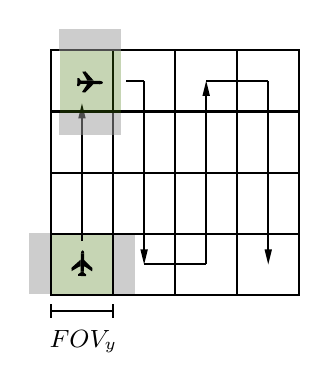
\begin{tikzpicture}[x=0.75pt,y=0.75pt,yscale=-1,xscale=1]
			%uncomment if require: \path (0,300); %set diagram left start at 0, and has height of 300
			
			%Shape: Rectangle [id:dp036802263347778474] 
			\draw  [draw opacity=0][fill={rgb, 255:red, 65; green, 117; blue, 5 }  ,fill opacity=0.3 ] (91.4,162.11) -- (121.3,162.11) -- (121.3,191.57) -- (91.4,191.57) -- cycle ;
			%Shape: Chord [id:dp8311663081836851] 
			\draw  [draw opacity=0][fill={rgb, 255:red, 0; green, 0; blue, 0 }  ,fill opacity=1 ] (105.79,172.1) .. controls (105.79,172.1) and (105.79,172.1) .. (105.79,172.1) .. controls (105.8,171.29) and (106.18,170.63) .. (106.62,170.64) .. controls (107.06,170.66) and (107.41,171.32) .. (107.39,172.14) -- cycle ;
			%Shape: Rectangle [id:dp8012179965756234] 
			\draw  [draw opacity=0][fill={rgb, 255:red, 0; green, 0; blue, 0 }  ,fill opacity=1 ] (107.39,172.14) -- (107.23,180.82) -- (105.62,180.78) -- (105.78,172.1) -- cycle ;
			%Shape: Chord [id:dp46276085808629674] 
			\draw  [draw opacity=0][fill={rgb, 255:red, 0; green, 0; blue, 0 }  ,fill opacity=1 ] (107.23,180.82) .. controls (107.23,180.82) and (107.23,180.82) .. (107.23,180.82) .. controls (107.21,181.63) and (106.84,182.28) .. (106.4,182.27) .. controls (105.95,182.26) and (105.61,181.59) .. (105.62,180.78) -- cycle ;
			%Shape: Boxed Polygon [id:dp33577441359912386] 
			\draw  [draw opacity=0][fill={rgb, 255:red, 0; green, 0; blue, 0 }  ,fill opacity=1 ] (111.19,180.75) -- (107.86,178.55) -- (107.16,178.35) -- (107.21,175.15) -- (111.37,179.23) -- cycle ;
			%Shape: Boxed Polygon [id:dp4613372486056908] 
			\draw  [draw opacity=0][fill={rgb, 255:red, 0; green, 0; blue, 0 }  ,fill opacity=1 ] (101.36,180.59) -- (104.88,178.52) -- (105.61,178.35) -- (105.65,175.11) -- (101.22,179.05) -- cycle ;
			%Shape: Boxed Polygon [id:dp09882619727387199] 
			\draw  [draw opacity=0][fill={rgb, 255:red, 0; green, 0; blue, 0 }  ,fill opacity=1 ] (108.27,182.2) -- (108.23,183.06) -- (104.44,182.93) -- (104.47,182.1) -- (106.42,180.8) -- cycle ;
			
			%Shape: Rectangle [id:dp43518650932458014] 
			\draw  [draw opacity=0][fill={rgb, 255:red, 155; green, 155; blue, 155 }  ,fill opacity=0.5 ] (121.3,162.07) -- (132.06,162.07) -- (132.06,191.61) -- (121.3,191.61) -- cycle ;
			%Shape: Rectangle [id:dp898186670672066] 
			\draw  [draw opacity=0][fill={rgb, 255:red, 155; green, 155; blue, 155 }  ,fill opacity=0.5 ] (80.64,162.07) -- (91.4,162.07) -- (91.4,191.61) -- (80.64,191.61) -- cycle ;
			
			%Shape: Rectangle [id:dp12911688161174095] 
			\draw   (91.4,74.26) -- (121.3,74.26) -- (121.3,103.72) -- (91.4,103.72) -- cycle ;
			%Shape: Rectangle [id:dp778307202398685] 
			\draw   (121.3,74.26) -- (151.2,74.26) -- (151.2,103.72) -- (121.3,103.72) -- cycle ;
			%Shape: Rectangle [id:dp5920975737411569] 
			\draw   (151.2,74.26) -- (181.1,74.26) -- (181.1,103.72) -- (151.2,103.72) -- cycle ;
			%Shape: Rectangle [id:dp7108929033014086] 
			\draw   (91.4,103.72) -- (121.3,103.72) -- (121.3,133.18) -- (91.4,133.18) -- cycle ;
			%Shape: Rectangle [id:dp8152064023887235] 
			\draw   (91.4,133.18) -- (121.3,133.18) -- (121.3,162.64) -- (91.4,162.64) -- cycle ;
			%Shape: Rectangle [id:dp01596026185419297] 
			\draw   (181.1,162.64) -- (211,162.64) -- (211,192.11) -- (181.1,192.11) -- cycle ;
			%Shape: Rectangle [id:dp7327882569457931] 
			\draw   (121.3,103.72) -- (151.2,103.72) -- (151.2,133.18) -- (121.3,133.18) -- cycle ;
			%Shape: Rectangle [id:dp11348064360337196] 
			\draw   (121.3,133.18) -- (151.2,133.18) -- (151.2,162.64) -- (121.3,162.64) -- cycle ;
			%Shape: Rectangle [id:dp5274571336670886] 
			\draw   (151.2,133.18) -- (181.1,133.18) -- (181.1,162.64) -- (151.2,162.64) -- cycle ;
			%Shape: Rectangle [id:dp1361244585482333] 
			\draw   (151.2,103.72) -- (181.1,103.72) -- (181.1,133.18) -- (151.2,133.18) -- cycle ;
			%Shape: Rectangle [id:dp8698952772815938] 
			\draw   (91.4,162.64) -- (121.3,162.64) -- (121.3,192.11) -- (91.4,192.11) -- cycle ;
			%Shape: Rectangle [id:dp8275138362077274] 
			\draw   (121.3,162.64) -- (151.2,162.64) -- (151.2,192.11) -- (121.3,192.11) -- cycle ;
			%Shape: Rectangle [id:dp5045016465037775] 
			\draw   (151.2,162.64) -- (181.1,162.64) -- (181.1,192.11) -- (151.2,192.11) -- cycle ;
			%Shape: Rectangle [id:dp5051198991702088] 
			\draw   (181.1,133.18) -- (211,133.18) -- (211,162.64) -- (181.1,162.64) -- cycle ;
			%Shape: Rectangle [id:dp9607013415516779] 
			\draw   (181.1,103.72) -- (211,103.72) -- (211,133.18) -- (181.1,133.18) -- cycle ;
			%Shape: Rectangle [id:dp5794670437040133] 
			\draw   (181.1,74.26) -- (211,74.26) -- (211,103.72) -- (181.1,103.72) -- cycle ;
			%Straight Lines [id:da9321367214575229] 
			\draw    (106.29,166.14) -- (106.29,101.86) ;
			\draw [shift={(106.29,99.86)}, rotate = 450] [fill={rgb, 255:red, 0; green, 0; blue, 0 }  ][line width=0.08]  [draw opacity=0] (7.2,-1.8) -- (0,0) -- (7.2,1.8) -- cycle    ;
			%Straight Lines [id:da40799678234401227] 
			\draw    (166.15,177.38) -- (166.15,90.99) ;
			\draw [shift={(166.15,88.99)}, rotate = 450] [fill={rgb, 255:red, 0; green, 0; blue, 0 }  ][line width=0.08]  [draw opacity=0] (7.2,-1.8) -- (0,0) -- (7.2,1.8) -- cycle    ;
			%Straight Lines [id:da2047551510485104] 
			\draw    (136.25,89.23) -- (127.29,89.23) ;
			%Shape: Rectangle [id:dp8051835391549806] 
			\draw  [draw opacity=0][fill={rgb, 255:red, 65; green, 117; blue, 5 }  ,fill opacity=0.3 ] (124.94,74.61) -- (124.94,104.51) -- (95.48,104.51) -- (95.48,74.61) -- cycle ;
			%Shape: Chord [id:dp01440978675599247] 
			\draw  [draw opacity=0][fill={rgb, 255:red, 0; green, 0; blue, 0 }  ,fill opacity=1 ] (114.95,88.99) .. controls (114.95,88.99) and (114.95,88.99) .. (114.95,88.99) .. controls (115.76,89.01) and (116.42,89.38) .. (116.4,89.83) .. controls (116.39,90.27) and (115.72,90.61) .. (114.91,90.6) -- cycle ;
			%Shape: Rectangle [id:dp47820815125081073] 
			\draw  [draw opacity=0][fill={rgb, 255:red, 0; green, 0; blue, 0 }  ,fill opacity=1 ] (114.91,90.6) -- (106.23,90.43) -- (106.27,88.82) -- (114.95,88.99) -- cycle ;
			%Shape: Chord [id:dp5606590464537962] 
			\draw  [draw opacity=0][fill={rgb, 255:red, 0; green, 0; blue, 0 }  ,fill opacity=1 ] (106.23,90.43) .. controls (105.42,90.42) and (104.77,90.05) .. (104.78,89.6) .. controls (104.79,89.16) and (105.46,88.81) .. (106.27,88.83) -- cycle ;
			%Shape: Boxed Polygon [id:dp9266491051896144] 
			\draw  [draw opacity=0][fill={rgb, 255:red, 0; green, 0; blue, 0 }  ,fill opacity=1 ] (106.3,94.4) -- (108.5,91.06) -- (108.7,90.37) -- (111.9,90.42) -- (107.82,94.58) -- cycle ;
			%Shape: Boxed Polygon [id:dp034397174811206854] 
			\draw  [draw opacity=0][fill={rgb, 255:red, 0; green, 0; blue, 0 }  ,fill opacity=1 ] (106.46,84.57) -- (108.53,88.09) -- (108.7,88.81) -- (111.94,88.86) -- (108,84.43) -- cycle ;
			%Shape: Boxed Polygon [id:dp03511489675126511] 
			\draw  [draw opacity=0][fill={rgb, 255:red, 0; green, 0; blue, 0 }  ,fill opacity=1 ] (104.85,91.48) -- (103.99,91.43) -- (104.12,87.65) -- (104.95,87.68) -- (106.25,89.63) -- cycle ;
			
			%Shape: Rectangle [id:dp6507888601892564] 
			\draw  [draw opacity=0][fill={rgb, 255:red, 155; green, 155; blue, 155 }  ,fill opacity=0.5 ] (124.98,104.51) -- (124.98,115.27) -- (95.44,115.27) -- (95.44,104.51) -- cycle ;
			%Shape: Rectangle [id:dp5268420170616126] 
			\draw  [draw opacity=0][fill={rgb, 255:red, 155; green, 155; blue, 155 }  ,fill opacity=0.5 ] (124.98,63.84) -- (124.98,74.61) -- (95.44,74.61) -- (95.44,63.84) -- cycle ;
			
			%Straight Lines [id:da6678654382408558] 
			\draw    (166.15,177.38) -- (136.25,177.38) ;
			%Straight Lines [id:da2744825079592068] 
			\draw    (166.15,88.99) -- (196.05,88.99) ;
			%Straight Lines [id:da1430427767977791] 
			\draw    (196.05,88.99) -- (196.05,175.38) ;
			\draw [shift={(196.05,177.38)}, rotate = 270] [fill={rgb, 255:red, 0; green, 0; blue, 0 }  ][line width=0.08]  [draw opacity=0] (7.2,-1.8) -- (0,0) -- (7.2,1.8) -- cycle    ;
			%Straight Lines [id:da45865584522885094] 
			\draw    (136.25,88.99) -- (136.25,175.38) ;
			\draw [shift={(136.25,177.38)}, rotate = 270] [fill={rgb, 255:red, 0; green, 0; blue, 0 }  ][line width=0.08]  [draw opacity=0] (7.2,-1.8) -- (0,0) -- (7.2,1.8) -- cycle    ;
			%Straight Lines [id:da8017813803709761] 
			\draw    (91.4,200) -- (121.4,200) ;
			\draw [shift={(121.4,200)}, rotate = 180] [color={rgb, 255:red, 0; green, 0; blue, 0 }  ][line width=0.75]    (0,3.35) -- (0,-3.35)   ;
			\draw [shift={(91.4,200)}, rotate = 180] [color={rgb, 255:red, 0; green, 0; blue, 0 }  ][line width=0.75]    (0,3.35) -- (0,-3.35)   ;
			
			% Text Node
			\draw (89.2,207.6) node [anchor=north west][inner sep=0.75pt]  [font=\small]  {$FOV_{y}$};
			
		\end{tikzpicture}
		\caption{Square discretisation}
		\label{fig:Overlap-sqr}
	\end{subfigure}
	\hfill
	\begin{subfigure}[b]{0.6\textwidth}
		\centering
		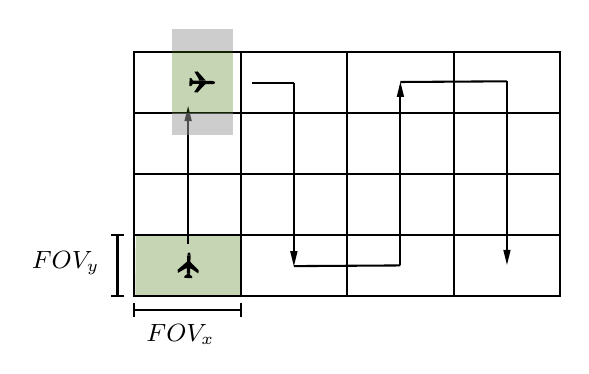
\begin{tikzpicture}[x=0.75pt,y=0.75pt,yscale=-1,xscale=1]
			%uncomment if require: \path (0,300); %set diagram left start at 0, and has height of 300
			
			%Shape: Rectangle [id:dp1592240079509375] 
			\draw  [draw opacity=0][fill={rgb, 255:red, 65; green, 117; blue, 5 }  ,fill opacity=0.3 ] (256.84,181.82) -- (307.71,182.34) -- (307.41,211.8) -- (256.54,211.29) -- cycle ;
			%Shape: Chord [id:dp027006860973721514] 
			\draw  [draw opacity=0][fill={rgb, 255:red, 0; green, 0; blue, 0 }  ,fill opacity=1 ] (281.6,192.06) .. controls (281.62,191.24) and (282,190.6) .. (282.44,190.61) .. controls (282.88,190.63) and (283.22,191.3) .. (283.2,192.11) -- cycle ;
			%Shape: Rectangle [id:dp5979870900127169] 
			\draw  [draw opacity=0][fill={rgb, 255:red, 0; green, 0; blue, 0 }  ,fill opacity=1 ] (283.2,192.11) -- (282.95,200.79) -- (281.34,200.73) -- (281.59,192.06) -- cycle ;
			%Shape: Chord [id:dp2765435991887346] 
			\draw  [draw opacity=0][fill={rgb, 255:red, 0; green, 0; blue, 0 }  ,fill opacity=1 ] (282.95,200.79) .. controls (282.92,201.6) and (282.54,202.25) .. (282.1,202.24) .. controls (281.66,202.22) and (281.32,201.55) .. (281.34,200.73) -- cycle ;
			%Shape: Boxed Polygon [id:dp6872706935659367] 
			\draw  [draw opacity=0][fill={rgb, 255:red, 0; green, 0; blue, 0 }  ,fill opacity=1 ] (286.91,200.76) -- (283.6,198.53) -- (282.91,198.32) -- (282.99,195.12) -- (287.11,199.24) -- cycle ;
			%Shape: Boxed Polygon [id:dp5311750689290109] 
			\draw  [draw opacity=0][fill={rgb, 255:red, 0; green, 0; blue, 0 }  ,fill opacity=1 ] (277.09,200.5) -- (280.62,198.47) -- (281.35,198.31) -- (281.43,195.07) -- (276.96,198.96) -- cycle ;
			%Shape: Boxed Polygon [id:dp9447821201006807] 
			\draw  [draw opacity=0][fill={rgb, 255:red, 0; green, 0; blue, 0 }  ,fill opacity=1 ] (283.98,202.18) -- (283.92,203.04) -- (280.14,202.88) -- (280.18,202.05) -- (282.14,200.76) -- cycle ;
			
			
			%Shape: Rectangle [id:dp49983792011863337] 
			\draw   (255.97,94.15) -- (307.3,94.15) -- (307.3,123.51) -- (255.97,123.51) -- cycle ;
			%Shape: Rectangle [id:dp8807821798790052] 
			\draw   (307.3,94.15) -- (358.63,94.15) -- (358.63,123.51) -- (307.3,123.51) -- cycle ;
			%Shape: Rectangle [id:dp8181512728288265] 
			\draw   (358.63,94.15) -- (409.96,94.15) -- (409.96,123.51) -- (358.63,123.51) -- cycle ;
			%Shape: Rectangle [id:dp09547819591891549] 
			\draw   (255.97,123.51) -- (307.3,123.51) -- (307.3,152.86) -- (255.97,152.86) -- cycle ;
			%Shape: Rectangle [id:dp1985429505890559] 
			\draw   (255.97,152.86) -- (307.3,152.86) -- (307.3,182.22) -- (255.97,182.22) -- cycle ;
			%Shape: Rectangle [id:dp5422527345143757] 
			\draw   (409.96,182.22) -- (461.29,182.22) -- (461.29,211.57) -- (409.96,211.57) -- cycle ;
			%Shape: Rectangle [id:dp332416764045272] 
			\draw   (307.3,123.51) -- (358.63,123.51) -- (358.63,152.86) -- (307.3,152.86) -- cycle ;
			%Shape: Rectangle [id:dp36287337689551014] 
			\draw   (307.3,152.86) -- (358.63,152.86) -- (358.63,182.22) -- (307.3,182.22) -- cycle ;
			%Shape: Rectangle [id:dp4697135024528536] 
			\draw   (358.63,152.86) -- (409.96,152.86) -- (409.96,182.22) -- (358.63,182.22) -- cycle ;
			%Shape: Rectangle [id:dp1298855569227555] 
			\draw   (358.63,123.51) -- (409.96,123.51) -- (409.96,152.86) -- (358.63,152.86) -- cycle ;
			%Shape: Rectangle [id:dp8663339040779854] 
			\draw   (255.97,182.22) -- (307.3,182.22) -- (307.3,211.57) -- (255.97,211.57) -- cycle ;
			%Shape: Rectangle [id:dp9437211813054305] 
			\draw   (307.3,182.22) -- (358.63,182.22) -- (358.63,211.57) -- (307.3,211.57) -- cycle ;
			%Shape: Rectangle [id:dp810113535837834] 
			\draw   (358.63,182.22) -- (409.96,182.22) -- (409.96,211.57) -- (358.63,211.57) -- cycle ;
			%Shape: Rectangle [id:dp5562129843015806] 
			\draw   (409.96,152.86) -- (461.29,152.86) -- (461.29,182.22) -- (409.96,182.22) -- cycle ;
			%Shape: Rectangle [id:dp8187981325254521] 
			\draw   (409.96,123.51) -- (461.29,123.51) -- (461.29,152.86) -- (409.96,152.86) -- cycle ;
			%Shape: Rectangle [id:dp6245482862531306] 
			\draw   (409.96,94.15) -- (461.29,94.15) -- (461.29,123.51) -- (409.96,123.51) -- cycle ;
			
			%Straight Lines [id:da41795839579175675] 
			\draw    (282,186.43) -- (282,122.14) ;
			\draw [shift={(282,120.14)}, rotate = 450] [fill={rgb, 255:red, 0; green, 0; blue, 0 }  ][line width=0.08]  [draw opacity=0] (7.2,-1.8) -- (0,0) -- (7.2,1.8) -- cycle    ;
			%Straight Lines [id:da1509716304633384] 
			\draw    (332.96,108.83) -- (312.68,108.83) ;
			%Straight Lines [id:da48049309446832655] 
			\draw    (332.96,108.83) -- (332.96,195.22) ;
			\draw [shift={(332.96,197.22)}, rotate = 270] [fill={rgb, 255:red, 0; green, 0; blue, 0 }  ][line width=0.08]  [draw opacity=0] (7.2,-1.8) -- (0,0) -- (7.2,1.8) -- cycle    ;
			%Straight Lines [id:da4231981271606413] 
			\draw    (384.29,196.89) -- (332.96,197.22) ;
			%Straight Lines [id:da4546308979435414] 
			\draw    (384.29,196.89) -- (384.29,110.51) ;
			\draw [shift={(384.29,108.51)}, rotate = 450] [fill={rgb, 255:red, 0; green, 0; blue, 0 }  ][line width=0.08]  [draw opacity=0] (7.2,-1.8) -- (0,0) -- (7.2,1.8) -- cycle    ;
			%Straight Lines [id:da10063088031705991] 
			\draw    (435.62,108.18) -- (384.29,108.51) ;
			%Straight Lines [id:da8147890256777217] 
			\draw    (435.62,108.18) -- (435.62,194.57) ;
			\draw [shift={(435.62,196.57)}, rotate = 270] [fill={rgb, 255:red, 0; green, 0; blue, 0 }  ][line width=0.08]  [draw opacity=0] (7.2,-1.8) -- (0,0) -- (7.2,1.8) -- cycle    ;
			%Shape: Rectangle [id:dp7310476894921445] 
			\draw  [draw opacity=0][fill={rgb, 255:red, 65; green, 117; blue, 5 }  ,fill opacity=0.3 ] (303.54,93.61) -- (303.54,123.51) -- (274.08,123.51) -- (274.08,93.61) -- cycle ;
			%Shape: Chord [id:dp19645121488474926] 
			\draw  [draw opacity=0][fill={rgb, 255:red, 0; green, 0; blue, 0 }  ,fill opacity=1 ] (293.55,107.99) .. controls (294.36,108.01) and (295.02,108.38) .. (295,108.83) .. controls (294.99,109.27) and (294.32,109.61) .. (293.51,109.6) -- cycle ;
			%Shape: Rectangle [id:dp05174583825785106] 
			\draw  [draw opacity=0][fill={rgb, 255:red, 0; green, 0; blue, 0 }  ,fill opacity=1 ] (293.51,109.6) -- (284.83,109.43) -- (284.87,107.82) -- (293.55,107.99) -- cycle ;
			%Shape: Chord [id:dp1661582095490599] 
			\draw  [draw opacity=0][fill={rgb, 255:red, 0; green, 0; blue, 0 }  ,fill opacity=1 ] (284.83,109.43) .. controls (284.02,109.42) and (283.37,109.05) .. (283.38,108.6) .. controls (283.39,108.16) and (284.06,107.81) .. (284.87,107.83) -- cycle ;
			%Shape: Boxed Polygon [id:dp018588797866418538] 
			\draw  [draw opacity=0][fill={rgb, 255:red, 0; green, 0; blue, 0 }  ,fill opacity=1 ] (284.9,113.4) -- (287.1,110.06) -- (287.3,109.37) -- (290.5,109.42) -- (286.42,113.58) -- cycle ;
			%Shape: Boxed Polygon [id:dp3166422244467362] 
			\draw  [draw opacity=0][fill={rgb, 255:red, 0; green, 0; blue, 0 }  ,fill opacity=1 ] (285.06,103.57) -- (287.13,107.09) -- (287.3,107.81) -- (290.54,107.86) -- (286.6,103.43) -- cycle ;
			%Shape: Boxed Polygon [id:dp7707267480495361] 
			\draw  [draw opacity=0][fill={rgb, 255:red, 0; green, 0; blue, 0 }  ,fill opacity=1 ] (283.45,110.48) -- (282.59,110.43) -- (282.72,106.65) -- (283.55,106.68) -- (284.85,108.63) -- cycle ;
			
			%Shape: Rectangle [id:dp26082048868605323] 
			\draw  [draw opacity=0][fill={rgb, 255:red, 155; green, 155; blue, 155 }  ,fill opacity=0.5 ] (303.58,123.51) -- (303.58,134.27) -- (274.04,134.27) -- (274.04,123.51) -- cycle ;
			%Shape: Rectangle [id:dp570071469284922] 
			\draw  [draw opacity=0][fill={rgb, 255:red, 155; green, 155; blue, 155 }  ,fill opacity=0.5 ] (303.58,82.84) -- (303.58,93.61) -- (274.04,93.61) -- (274.04,82.84) -- cycle ;
			
			%Straight Lines [id:da1628094381777676] 
			\draw    (247.97,182.22) -- (247.97,211.57) ;
			\draw [shift={(247.97,211.57)}, rotate = 270] [color={rgb, 255:red, 0; green, 0; blue, 0 }  ][line width=0.75]    (0,3.35) -- (0,-3.35)   ;
			\draw [shift={(247.97,182.22)}, rotate = 270] [color={rgb, 255:red, 0; green, 0; blue, 0 }  ][line width=0.75]    (0,3.35) -- (0,-3.35)   ;
			%Straight Lines [id:da97063001945603] 
			\draw    (255.97,218.57) -- (307.3,218.57) ;
			\draw [shift={(307.3,218.57)}, rotate = 180] [color={rgb, 255:red, 0; green, 0; blue, 0 }  ][line width=0.75]    (0,3.35) -- (0,-3.35)   ;
			\draw [shift={(255.97,218.57)}, rotate = 180] [color={rgb, 255:red, 0; green, 0; blue, 0 }  ][line width=0.75]    (0,3.35) -- (0,-3.35)   ;
			
			% Text Node
			\draw (260.4,223.8) node [anchor=north west][inner sep=0.75pt]  [font=\small]  {$FOV_{x}$};
			% Text Node
			\draw (205.2,188.6) node [anchor=north west][inner sep=0.75pt]  [font=\small]  {$FOV_{y}$};
			
			
		\end{tikzpicture}
		\caption{Rectangular discretisation}
		\label{fig:Overlap-rect}
	\end{subfigure}
	\caption{Diagrams showing cross track overlap for camera Field of View for different discretisation techniques.}
\end{figure}

% TODO: Section where it is applied to different camera scenarios
\section{Implementation with Different Cameras}
\label{sec:ER-App}
% mention how dynamic constraints change everything - with this discretisation the asumption is that UAV can make 90 degree turns. This may be possible for some UAVs, but not while maintaining a constant velocity. Maintaining constant is more desireable because it consumes less energy. Mention how it is covered in a later section.


